\chapter{Introduction} \label{ch: introduction}

\graphicspath{{01-introduction/figures/}}

\begin{chapterquote}[Lewis Carroll][Alice in Wonderland][Chapter XII]
  Begin at the beginning,'' the King said, very gravely,
  ``and go on till you come to the end: then stop.
\end{chapterquote}

In this introductory Chapter we briefly introduce the field of solar physics, after which we will elaborate a bit further on the sun itself. Some general terminology will be introduced while also discussing certain features observable in the solar atmosphere, since they are quite relevant in the scope of early Chapters. Eventually we bring waves and instabilities into play, as they are in essence a main topic in this thesis, and discuss their importance both in a solar physical context as well as in more general (astro)physical settings.

\section{A very brief history of astrophysics}
The wonderful field of astrophysics encompasses a plethora of different disciplines. Historically, astrophysics has its roots in astronomy, which is in itself a millennia-old science. Back in ancient Greece people were already wondering about various heavenly objects and how to explain their peculiar motions, and centuries later it was realised that these objects actually obey natural laws. Since then the field of astrophysics has greatly expanded, including not only observational astronomy, but also computational and theoretical astrophysics, quantum mechanics, nuclear physics and even chemistry; and the list has recently been expanded even further, now also including gravitational wave astronomy. All these fields are intricately linked, depending on the objects that are being studied. While historically astronomy ``only'' studied the motions of stars and planets, we now know that there are a myriad of fascinating objects all around us: stars actually exist in all sorts and sizes, depending on how far along they are in their evolutionary process; ranging from huge supergiants to regular sized stars such as the sun, to baby proto-stars that are not even ``born'' yet. The list can be further extended with planetary systems, nebulae, and more exotic objects such as neutron stars or black holes, with the latter typically being accompanied with high-energy jets.

\begin{figure}[t]
  \centering
  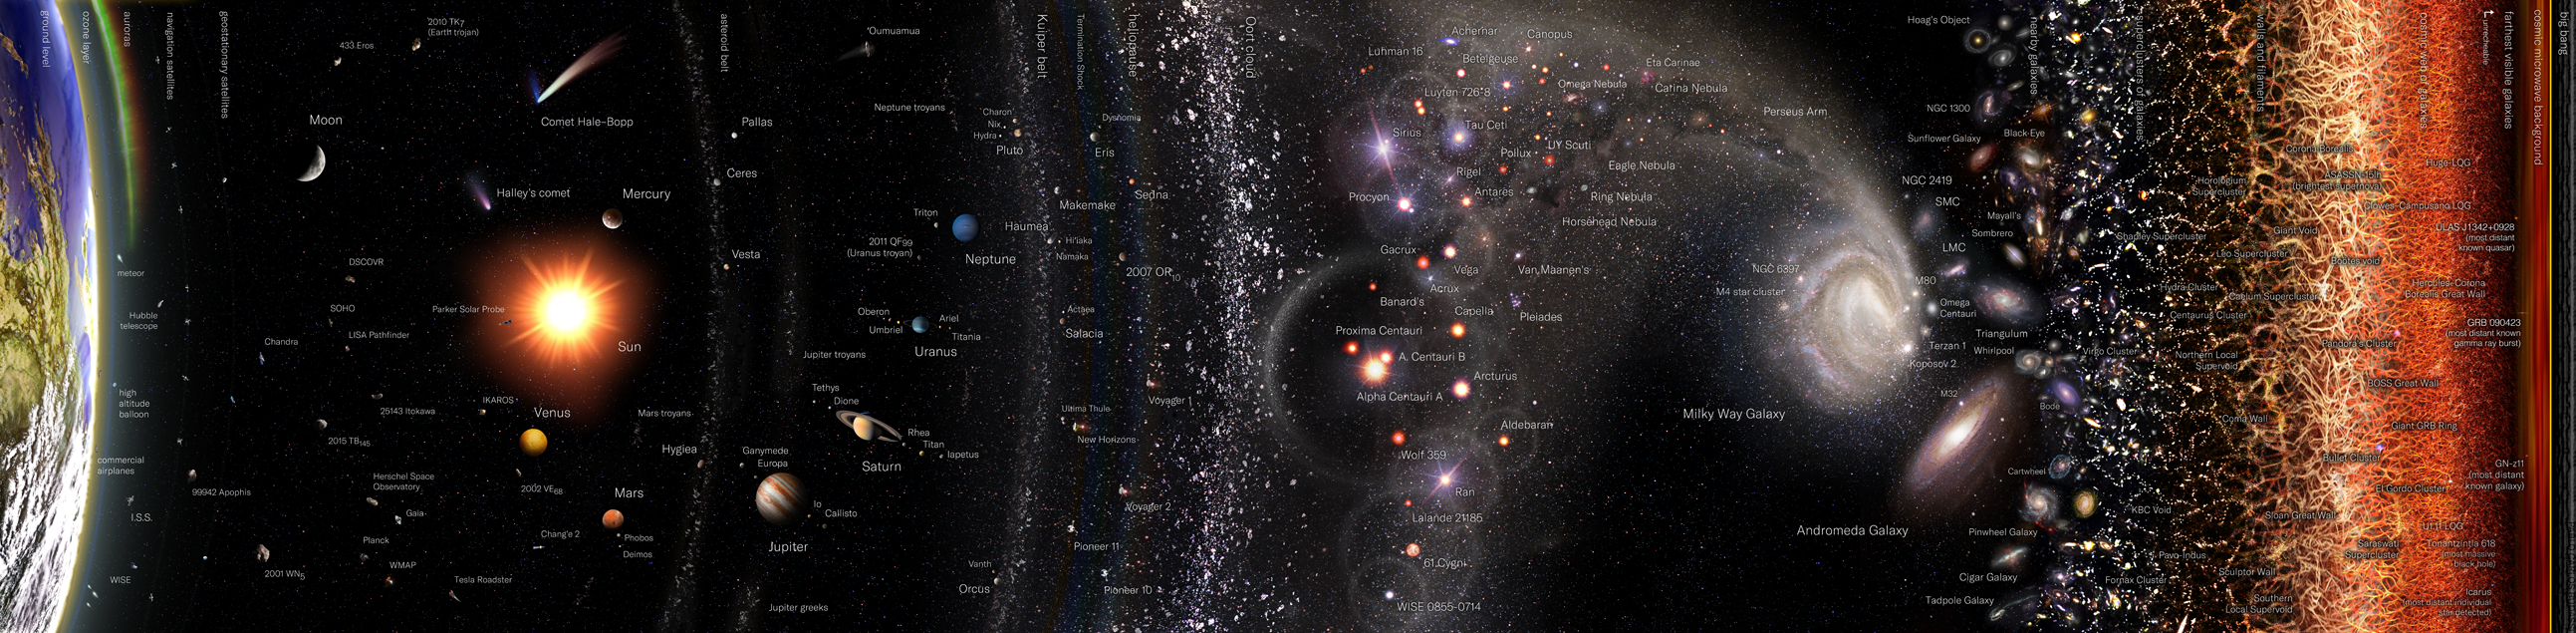
\includegraphics[width=\textwidth]{observable_universe.png}
  \caption{
    Artistic rendering of the observable universe, shown on a logarithmic scale from left to right based on proximity to Earth. Figure by Pablo Carlos Budassi.
  }
\end{figure}

In most (if not all) fields related to astrophysics research deals with \emph{plasma}, as it is by far the most abundant form of ordinary matter in the universe (we say ``ordinary'' here as we explicitly exclude dark matter and dark energy, whatever they might be). A plasma can be simplified as an ionised gas, hence a significant part of it are charged particles which in turn implies that electromagnetic fields are of extreme importance. Depending on the amount of neutral particles present a plasma can either be fully ionised (no neutrals) or partially ionised (some neutrals). In this thesis we only consider a fully ionised plasma, which will be quite sufficient for (most of) our applications.

The tools used to study astrophysics vary greatly, and similar to the various disciplines depend on which objects are being studied. In the time of Newton and Galilei tools mostly consisted of early telescopes and basic mathematical methods. Over the years new theories have been developed, where Einstein's general relativity is probably the most notable in an astrophysical context, which came accompanied with numerous advances and physical insights. From an observational viewpoint we evolved from using basic, simple telescopes to (arrays of) huge ground and space based telescopes and observatories designed to probe the deepest reaches of our universe. Additionally, with the advent of the computer age a completely new set of tools became available: suddenly it was possible to numerically solve systems of equations that were previously unsolvable using analytical methods, and this in turn sparked a whole new branch of computational astrophysics. Large-scale numerical codes have been developed since then, which can exploit a huge number of computational resources in parallel using the most powerful supercomputers on the planet. This has opened a completely new door into the wonderful world of astrophysics, where it is now possible to numerically probe and visualise even the most exotic astrophysical objects at extreme resolutions.

The field of solar physics studies, as the name suggests, our sun. Even here research topics are widely spread out, ranging from the solar interior to features on the solar surface, to the entire solar atmosphere and the link of the solar wind on space weather, to name a few. In this thesis we will mainly focus on waves and instability aspects from a spectroscopic standpoint, which can be directly linked to interesting structures in the solar atmosphere, that is, parts of the solar corona and chromosphere. We will mainly rely on numerical approaches, supplemented with a strong mathematical foundation.


\section{The Sun in a nutshell}
% briefly discuss the solar atmosphere, general structure, prominences, etc
% max 4 pages

\section{The importance of instabilities}
% discuss everyday role of waves and instabilities
% max 3 pages

\section{General outline}
% thesis outline summarised in 1 page


\cleardoublepage
